% !TEX encoding = UTF-8 Unicode
% !TEX root = DesignDocument.tex
\chapter{Release -- Setup -- Deployment}
This section will explain the setup and initialization of the Virtual Museum. It will be seperated into details about the hardware used to run the program, how to launch the program in exe, and launching in the Unreal Engine 4's Editor.


\section{Deployment Information and Dependencies}
Are there dependencies that are not embedded into the system install? 



\section{Setup Information}

\subsection{Occulus SDK Installation}
Before you can use the SDK, you need set up the drivers for your operating system. If your drivers are already set up, please skip to the  section. This content repeats the instructions in the Oculus Rift User Guide. The first thing to do is, download the Oculus Runtime Installer from the Oculus website. The Runtime is available from https://developer.oculus.com/downloads/.
\\ This will install the following components:
\\
\\Oculus Display Driver (Windows Only)
\\ Oculus Positional Tracking Sensor Driver
\\ Oculus Service Application
\\ Oculus System Tray Application and Configuration Utility Windows
\\

\subsection{Occulus Drivers-Windows}

This section describes how to install the Windows Runtime Package.
\\
\\To install the package:
\\
\\
Download the runtime from https://developer.oculus.com/downloads/. In the Windows Control Panel, go to Programs -> Programs and Features and uninstall any existing components. Run the install executable found in this package. This will install all the components described above and prompt you to restart your computer. Restart your computer. If you want to remove the Runtime package for the current user, run the provided Uninstaller or run the OculusDirectory/Agent/uninstallAgent.sh shell script from the command line.


\subsection{Occulus Drivers-Mac}

This section describe how to install the Mac Runtime Package.
\\
\\
To install the package:
\\
\\
Download the runtime from https://developer.oculus.com/downloads/. Run the installer application found inside the package. This will install all components described above for the current user only. You must run the installer for each user that wants to use the Rift.
Since the MacOS does not currently support direct rendering, you must adjust your display settings to rotate the display by 90 degrees for the Oculus Rift DK2. The display settings are located in System Preferences -> Displays. Additionally, consider disabling display mirroring via the Mirror Displays check box on the display adjustment tab.
If you want to remove the Runtime package for the current user, run the provided Uninstaller or run the OculusDirectory/Agent/uninstallAgent.sh shell script from the command line.

\subsection{Setting Up Occulus Rift Hardware}
This section will explain how to set up the Occulus using the SDK2.
Connect your DK2 headset to your computer, following the included Instruction Manual (which can also be found online).
Run the Oculus Configuration Utility by Right-clicking on the Oculus icon in the system tray and selecting Configuration Utility. When opened, the Oculus Configuration Utility will look like the following image.\\ 
\\
\begin{center}
\centering
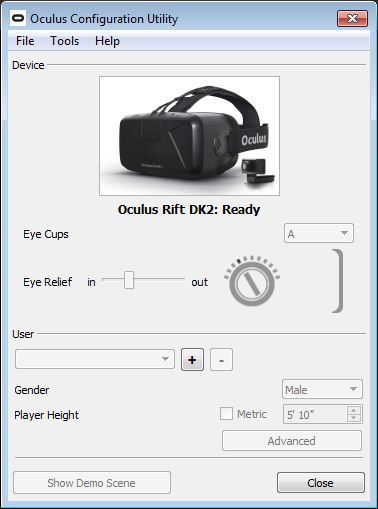
\includegraphics[scale=0.75]{Oculus_Config_Utility}\\
\end{center}
Under the User section press the Plus Sign to add a new User profile, as seen below\\
\begin{center}
\centering
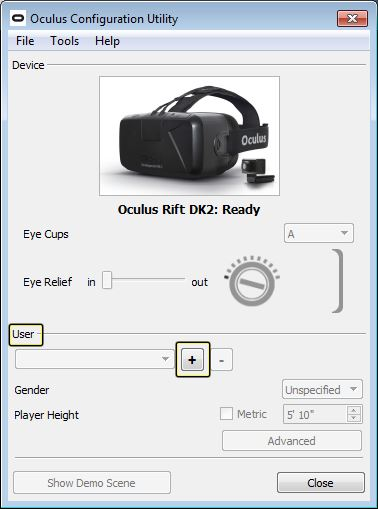
\includegraphics[scale=0.75]{Oculus_Config_Add_Profile}\\
\end{center}
In the New User pop up box that is displayed enter a name for the profile and then click the OK button.
\begin{center}
\centering
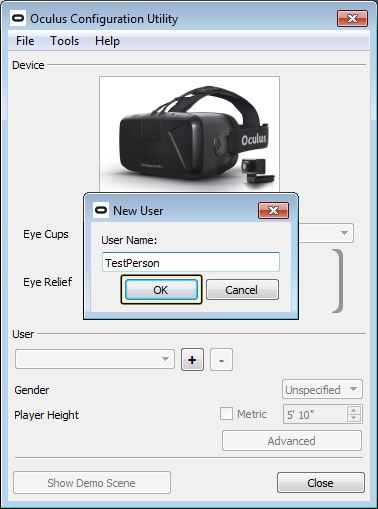
\includegraphics[scale=0.75]{Oculus_Config_Name_Profile}\\
\end{center}
Then set the in the User section set the Gender to the gender of the person using the Head Mounted Display(HMD) and set the Player Height to that persons height.
\begin{center}
\centering
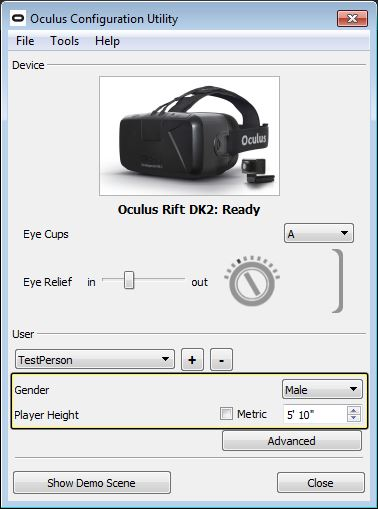
\includegraphics[scale=0.75]{Oculus_Config_Setup_Profile}\\
\end{center}
Click the Show Demo Scene button on the Oculus Configuration Utility and you should now see something similar to the following image being displayed on screen as well as being displayed in the HMD.S
\begin{center}
\centering
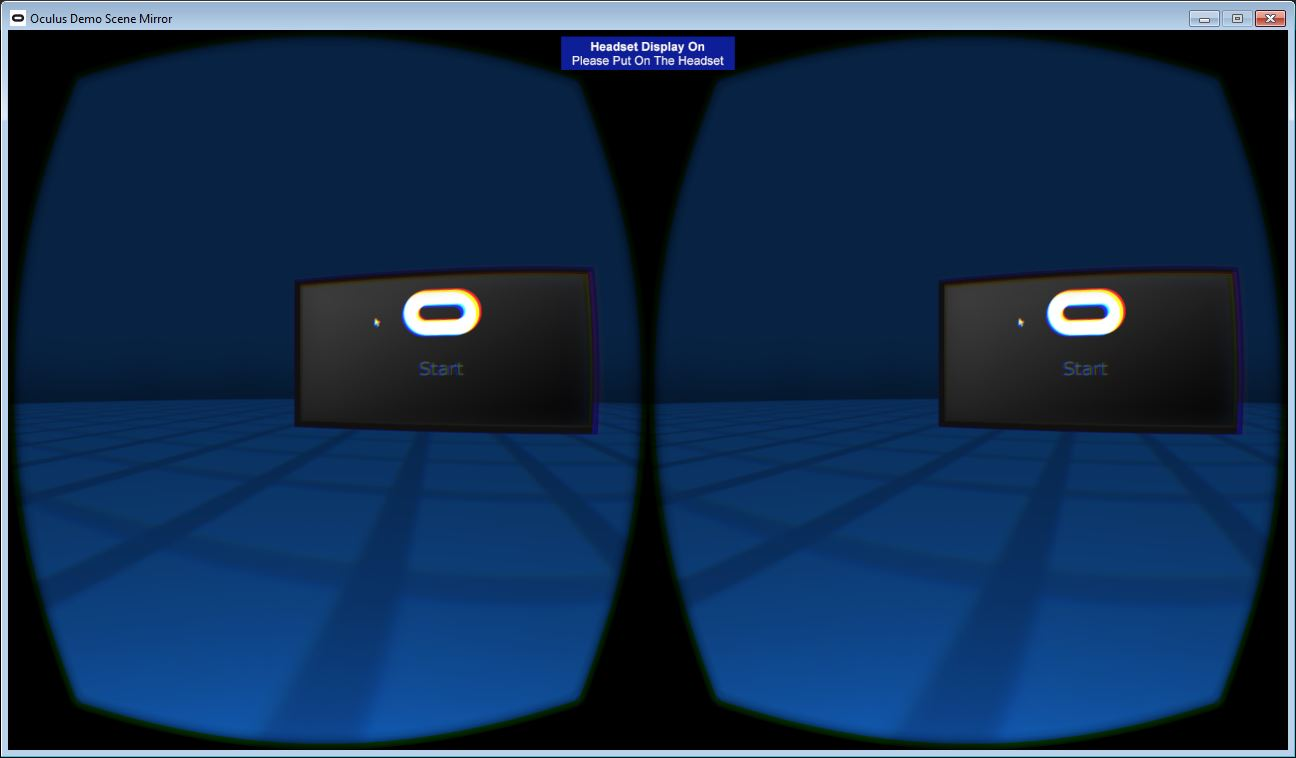
\includegraphics[scale=0.35]{Oculus_Config_Demo_Sceen}\\
\end{center}


\subsection{Unreal 4 Developement Engine}
This section will cover how to download the Unreal 4 Engine. First you will have to go to \url{https://www.unrealengine.com/what-is-unreal-engine-4} and click the get unreal button. It will then link you to  a create new user page, fill out the information and press create. The following page will then ask for a End User License Agreement. After reading it check the `I have read and agree to the End User License Agreement` check box, then click accept. It will then prompt a download button. After clicking this it will begin the downlaod for the Unreal Developement Engine.


\section{System  Versioning Information}

